\documentclass{article}
\usepackage{multirow}
\usepackage{color, colortbl}
\usepackage[first=0,last=9]{lcg}
\newcommand{\ra}{\rand0.\arabic{rand}}
\usepackage[a4paper,landscape]{geometry}
\usepackage[table]{xcolor}
\usepackage{multicol}
\usepackage[font=small,labelfont=bf]{caption}% newly added by me
\usepackage{palatino}
\usepackage{graphicx}
\graphicspath{{images/}}
\begin{document}

\begin{tabular*}{\linewidth}{@{}c|@{}c|@{}c|@{}c|@{}c|@{}c|@{}}
    {\hfill{} 1\hfill{}} & 
    {\hfill{} 2\hfill{}} &
    {\hfill{} 3\hfill{}} &
    {\hfill{} 4\hfill{}} &
    {\hfill{} 3\hfill{}} 
  \end{tabular*}
\begin{tabular}{@{}c@{ }c@{ }c@{ }c@{}}
    {\hfill{} 1\hfill{}} & 
    {\hfill{} 2\hfill{}} &
    {\hfill{} 3\hfill{}} &
    \end{tabular}

\begin{table}[htbp]
    \caption{Table with gray and white.}
    \begin{center}
    \begin{tabular}{cccccccccccccc}\rowcolor{lightgray}
   &&Jan&Feb&Mar&Apr&May&Jun&Jul&Aug&Sep&Oct&Nov&Dec\\
   \multicolumn{1}{>{\columncolor{lightgray}}l}{}& $\tau$ &0.305 **&0.312 **&0.163 **&0.0685&0.177 **&0.209 **&0.284**&0.297 **&0.375 **&0.265 **&0.335 **&0.362**\\                                \rowcolor{lightgray}
   \multicolumn{1}{>{\columncolor{lightgray}}l}{\multirow{-3}{*}{TAVG}}&R$^{2}$&0.219 **&0.209 **&0.069 **&0.017&0.074 **&0.106 **&0.151 **&0.205 **&0.306 **&0.152 **&0.226 **&0.244 **\\ 
   \multicolumn{1}{>{\columncolor{white}}l}{}& $\tau$&-0.227 **&-0.159 *& -0.176 **&-0.209 **& -0.252 **& -0.166 *& 0.307 **&0.102&0.258 **&0.0356& 0.303 **& 0.494**\\ \rowcolor{lightgray}
  \multicolumn{1}{>{\columncolor{white}}l}{\multirow{-3}{*}{TMAX}}&R$^{2}$&0.127 **& 0.069 **& 0.061 **& 0.088 **& 0.112 **& 0.047 *& 0.221 **&0.034& 0.129 **&0.001& 0.177 **& 0.47 **\\
   \multicolumn{1}{>{\columncolor{lightgray}}l}{}& $\tau$&-0.303 **&-0.00551&  -0.15 *&  -0.194 **&  -0.365 **&  -0.226 **&  -0.141 *&-0.0359&  0.271 **&  -0.434 **&-0.215 **& -0.17**\\\rowcolor{lightgray}
  \multicolumn{1}{>{\columncolor{lightgray}}l}{\multirow{-3}{*}{TMIN}}&R$^{2}$&0.276 **&0& 0.043 *& 0.075 **& 0.302 **& 0.097 **& 0.049 *&0.006& 0.167 **& 0.381 **& 0.118 **& 0.057 *\\
    \end{tabular}
    \end{center}
    \end{table}
%\begin{table}[htbp]
   \begin{tabular}{ccccc}\rowcolor{lightgray}
   STATIONS&& TMAX & TMIN & TAVG\\
\multicolumn{1}{>{\columncolor{white}}l}{}&Average($^\circ$ C)&31.6$\pm$1.12&18.1$\pm$1.21&27.4$\pm$0.80 \\ \rowcolor{lightgray} 
\multicolumn{1}{>{\columncolor{white}}l}{\multirow{-3}{*}{SURAT}}&$\tau$&0.013&0.032&0.028\\
\multicolumn{1}{>{\columncolor{lightgray}}l}{}&Average($^\circ$ C)&31.9$\pm$1.03&22.6$\pm$0.85&27.1$\pm$0.85 \\ \rowcolor{lightgray} 
\multicolumn{1}{>{\columncolor{lightgray}}l}{\multirow{-3}{*}{BOMBAY/SANTACRUZ}}&$\tau$&0.338**&0&0.288**\\
\multicolumn{1}{>{\columncolor{white}}l}{}&Average($^\circ$ C)&31.7$\pm$0.82&23.9$\pm$0.73&27.3$\pm$0.75 \\ \rowcolor{lightgray} 
\multicolumn{1}{>{\columncolor{white}}l}{\multirow{-3}{*}{BOMBAY / COLA}}&$\tau$&0.062&0.217**&0.283**\\
\multicolumn{1}{>{\columncolor{lightgray}}l}{}&Average($^\circ$ C)&31.5$\pm$1.08&18.0$\pm$1.56&24.9$\pm$0.91 \\ \rowcolor{lightgray} 
\multicolumn{1}{>{\columncolor{lightgray}}l}{\multirow{-3}{*}{PUNE}}&$\tau$&0.185**&0&-0.04**\\
\multicolumn{1}{>{\columncolor{white}}l}{}&Average($^\circ$ C)&30.1$\pm$0.87&22.2$\pm$0.81&26.8$\pm$0.67 \\ \rowcolor{lightgray} 
\multicolumn{1}{>{\columncolor{white}}l}{\multirow{-3}{*}{RATNAGIRI}}&$\tau$&0.212**&-0.13**&0.03\\
\multicolumn{1}{>{\columncolor{lightgray}}l}{}&Average($^\circ$ C)&30.2$\pm$0.96&18.4$\pm$1.04&24.3$\pm$0.67 \\ \rowcolor{lightgray} 
\multicolumn{1}{>{\columncolor{lightgray}}l}{\multirow{-3}{*}{BELGAUM/SAMBRA}}&$\tau$&0.241**&-0.08**&0.058\\
\multicolumn{1}{>{\columncolor{white}}l}{}&Average($^\circ$ C)&$\pm$&$\pm$&24.2$\pm$0.84 \\ \rowcolor{lightgray} 
\multicolumn{1}{>{\columncolor{white}}l}{\multirow{-3}{*}{BELGAUM}}&$\tau$&&&0.342**\\
\multicolumn{1}{>{\columncolor{lightgray}}l}{}&Average($^\circ$ C)&31.6$\pm$0.79&23.4$\pm$0.75&27.4$\pm$0.66 \\ \rowcolor{lightgray} 
\multicolumn{1}{>{\columncolor{lightgray}}l}{\multirow{-3}{*}{GOA/PANJI}}&$\tau$&0.241**&-0.01&0.222**\\
\multicolumn{1}{>{\columncolor{white}}l}{}&Average($^\circ$ C)&31.5$\pm$0.85&23.1$\pm$1.13&27.3$\pm$0.84 \\ \rowcolor{lightgray} 
\multicolumn{1}{>{\columncolor{white}}l}{\multirow{-3}{*}{NOVA GOA}}&$\tau$&-0.30**&-0.09**&-0.23**\\
\multicolumn{1}{>{\columncolor{lightgray}}l}{}&Average($^\circ$ C)&29.7$\pm$0.84&23.7$\pm$0.79&26.7$\pm$0.72 \\ \rowcolor{lightgray} 
\multicolumn{1}{>{\columncolor{lightgray}}l}{\multirow{-3}{*}{MARMAGAO}}&$\tau$&-0.14**&-0.07**&-0.11**\\
\multicolumn{1}{>{\columncolor{white}}l}{}&Average($^\circ$ C)&29.5$\pm$0.89&19.1$\pm$0.68&23.9$\pm$0.71 \\ \rowcolor{lightgray} 
\multicolumn{1}{>{\columncolor{white}}l}{\multirow{-3}{*}{BANGALORE}}&$\tau$&0.196**& 0.22**&0.267**\\
\multicolumn{1}{>{\columncolor{lightgray}}l}{}&Average($^\circ$ C)&31.7$\pm$0.73&23.0$\pm$0.6&27.0$\pm$0.58 \\ \rowcolor{lightgray} 
\multicolumn{1}{>{\columncolor{lightgray}}l}{\multirow{-3}{*}{MANGALORE/BAJPE}}&$\tau$&0.217**&-0.04&0.201**\\
\multicolumn{1}{>{\columncolor{white}}l}{}&Average($^\circ$ C)&30.5$\pm$0.68&23.5$\pm$0.67&27.0$\pm$0.61 \\ \rowcolor{lightgray} 
\multicolumn{1}{>{\columncolor{white}}l}{\multirow{-3}{*}{MANGALORE}}&$\tau$& 0.057*&0.124**&0.118**\\
\multicolumn{1}{>{\columncolor{lightgray}}l}{}&Average($^\circ$ C)&31.3$\pm$0.88&24.2$\pm$0.59&27.7$\pm$0.62 \\ \rowcolor{lightgray} 
\multicolumn{1}{>{\columncolor{lightgray}}l}{\multirow{-3}{*}{KOZHIKODE}}&$\tau$&0.499**&0.258**&0.396**\\
\multicolumn{1}{>{\columncolor{white}}l}{}&Average($^\circ$ C)&32.4$\pm$0.94&21.5$\pm$0.65&26.4$\pm$0.71 \\ \rowcolor{lightgray} 
\multicolumn{1}{>{\columncolor{white}}l}{\multirow{-3}{*}{COIMBATORE/PEELAMED}}&$\tau$& 0.082*&0.199**&0.156**\\
\multicolumn{1}{>{\columncolor{lightgray}}l}{}&Average($^\circ$ C)&31.1$\pm$0.69&24.2$\pm$0.59&27.3$\pm$0.54 \\ \rowcolor{lightgray} 
\multicolumn{1}{>{\columncolor{lightgray}}l}{\multirow{-3}{*}{FORT COCHIN}}&$\tau$& 0.084*& 0.087*&0.059**\\
\multicolumn{1}{>{\columncolor{white}}l}{}&Average($^\circ$ C)&31.4$\pm$0.89&23.6$\pm$0.47&27.0$\pm$0.68 \\ \rowcolor{lightgray} 
\multicolumn{1}{>{\columncolor{white}}l}{\multirow{-3}{*}{THIRUVANANTHAPURAM}}&$\tau$&0.429**&0.059&0.476**\\
   \end{tabular}
 
\begin{minipage}{\linewidth}
\centering
 
\label{tab:name}
 \begin{tabular}{@{}c@{ }}
    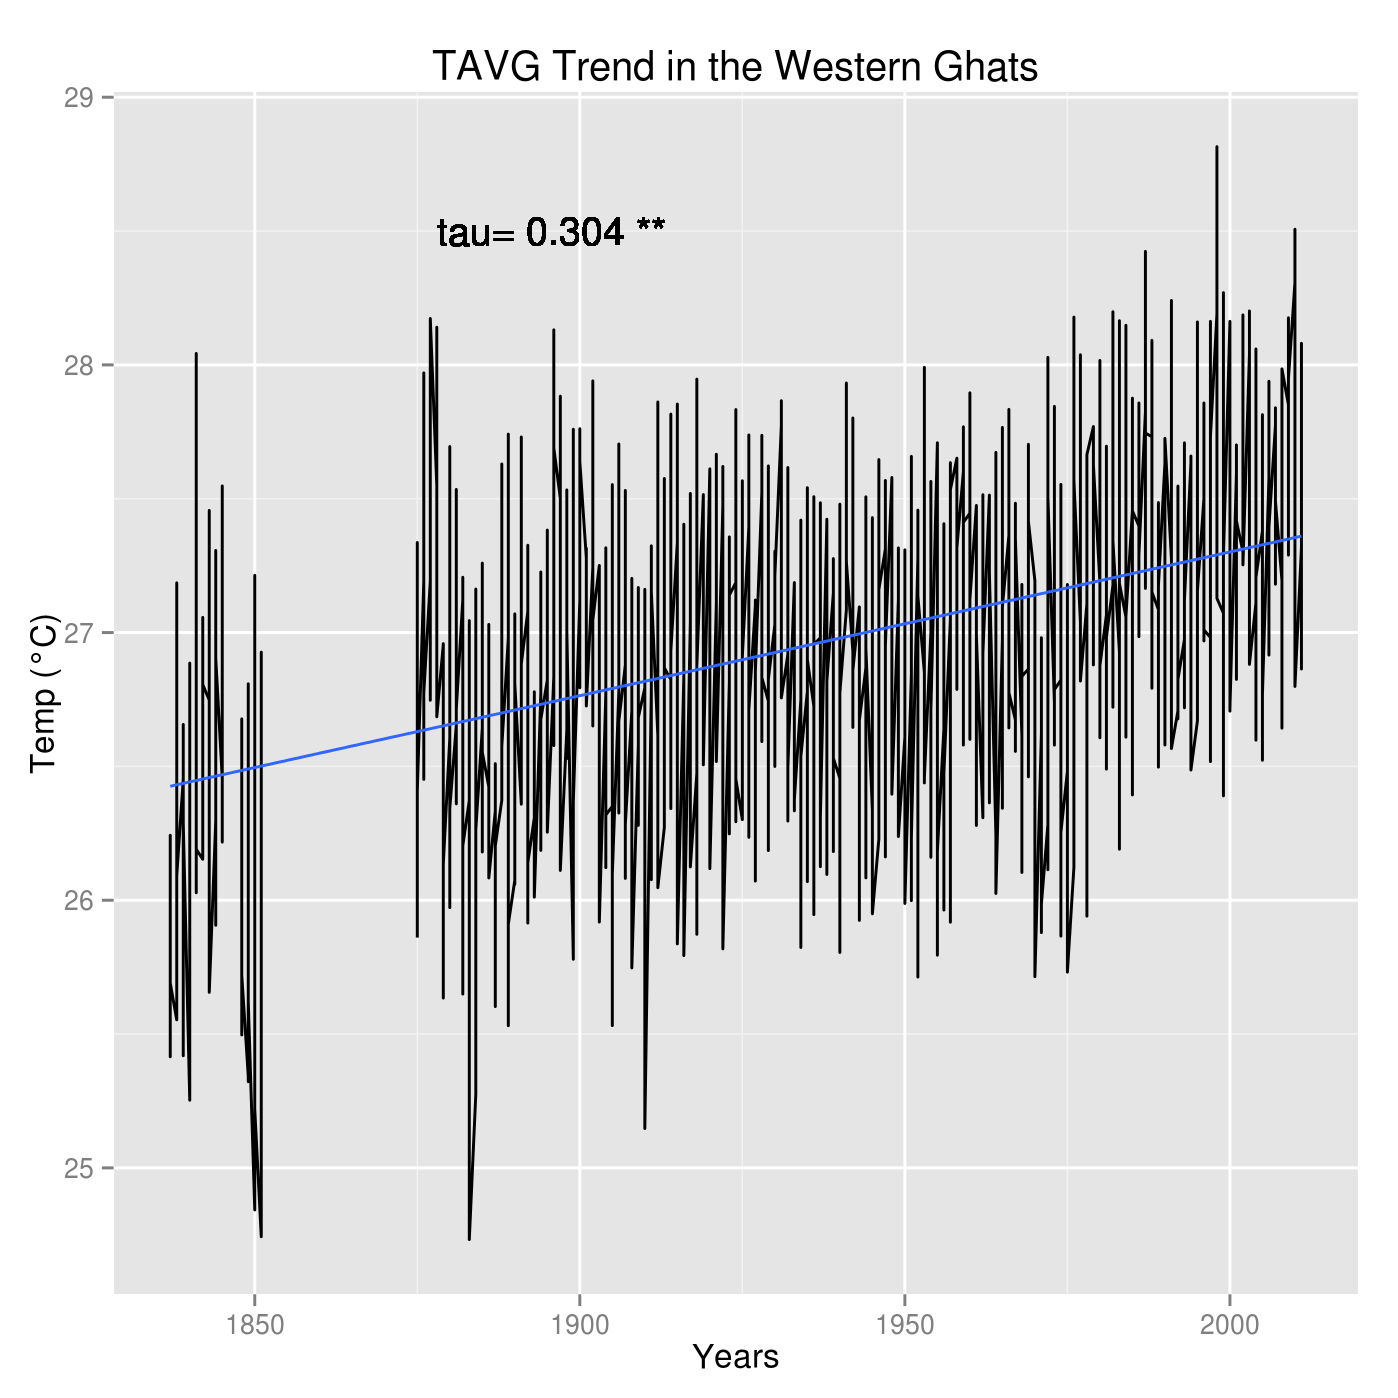
\includegraphics[width=5cm,height=2.7cm]{TAVG.png}\\
    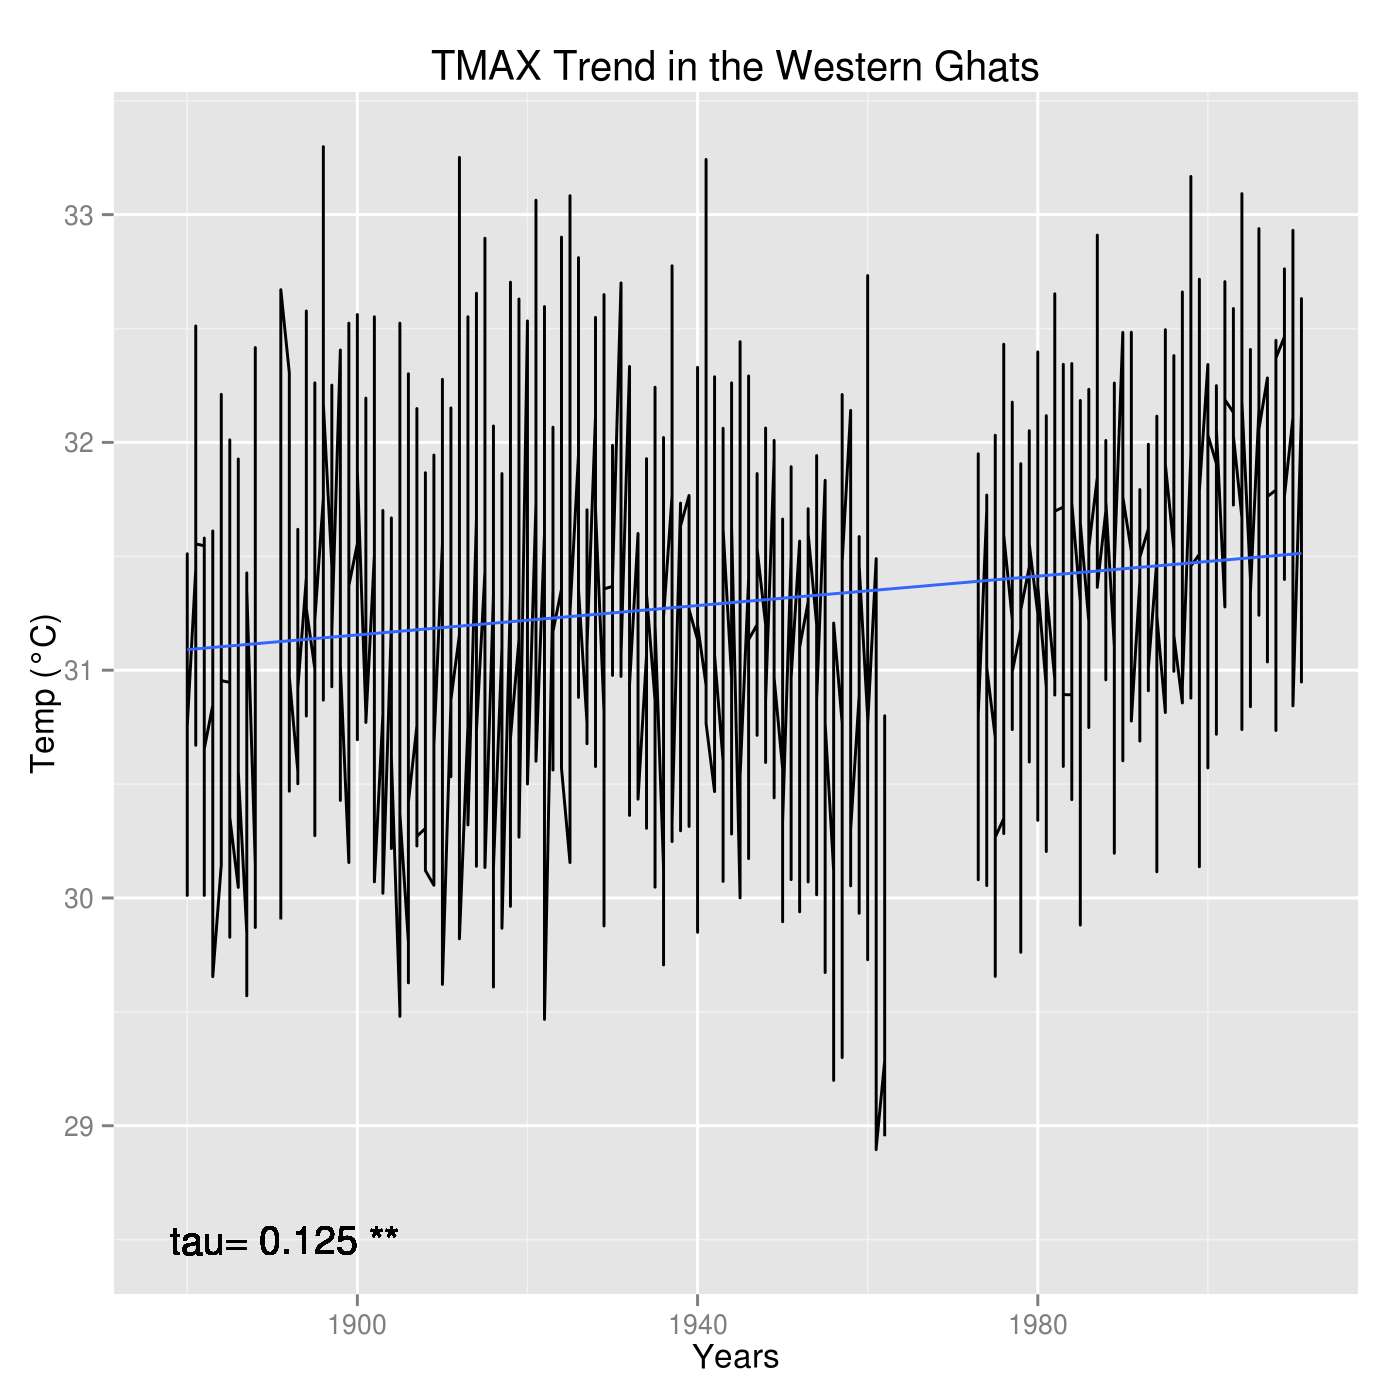
\includegraphics[width=5cm,height=2.7cm]{TMAX.png}\\
    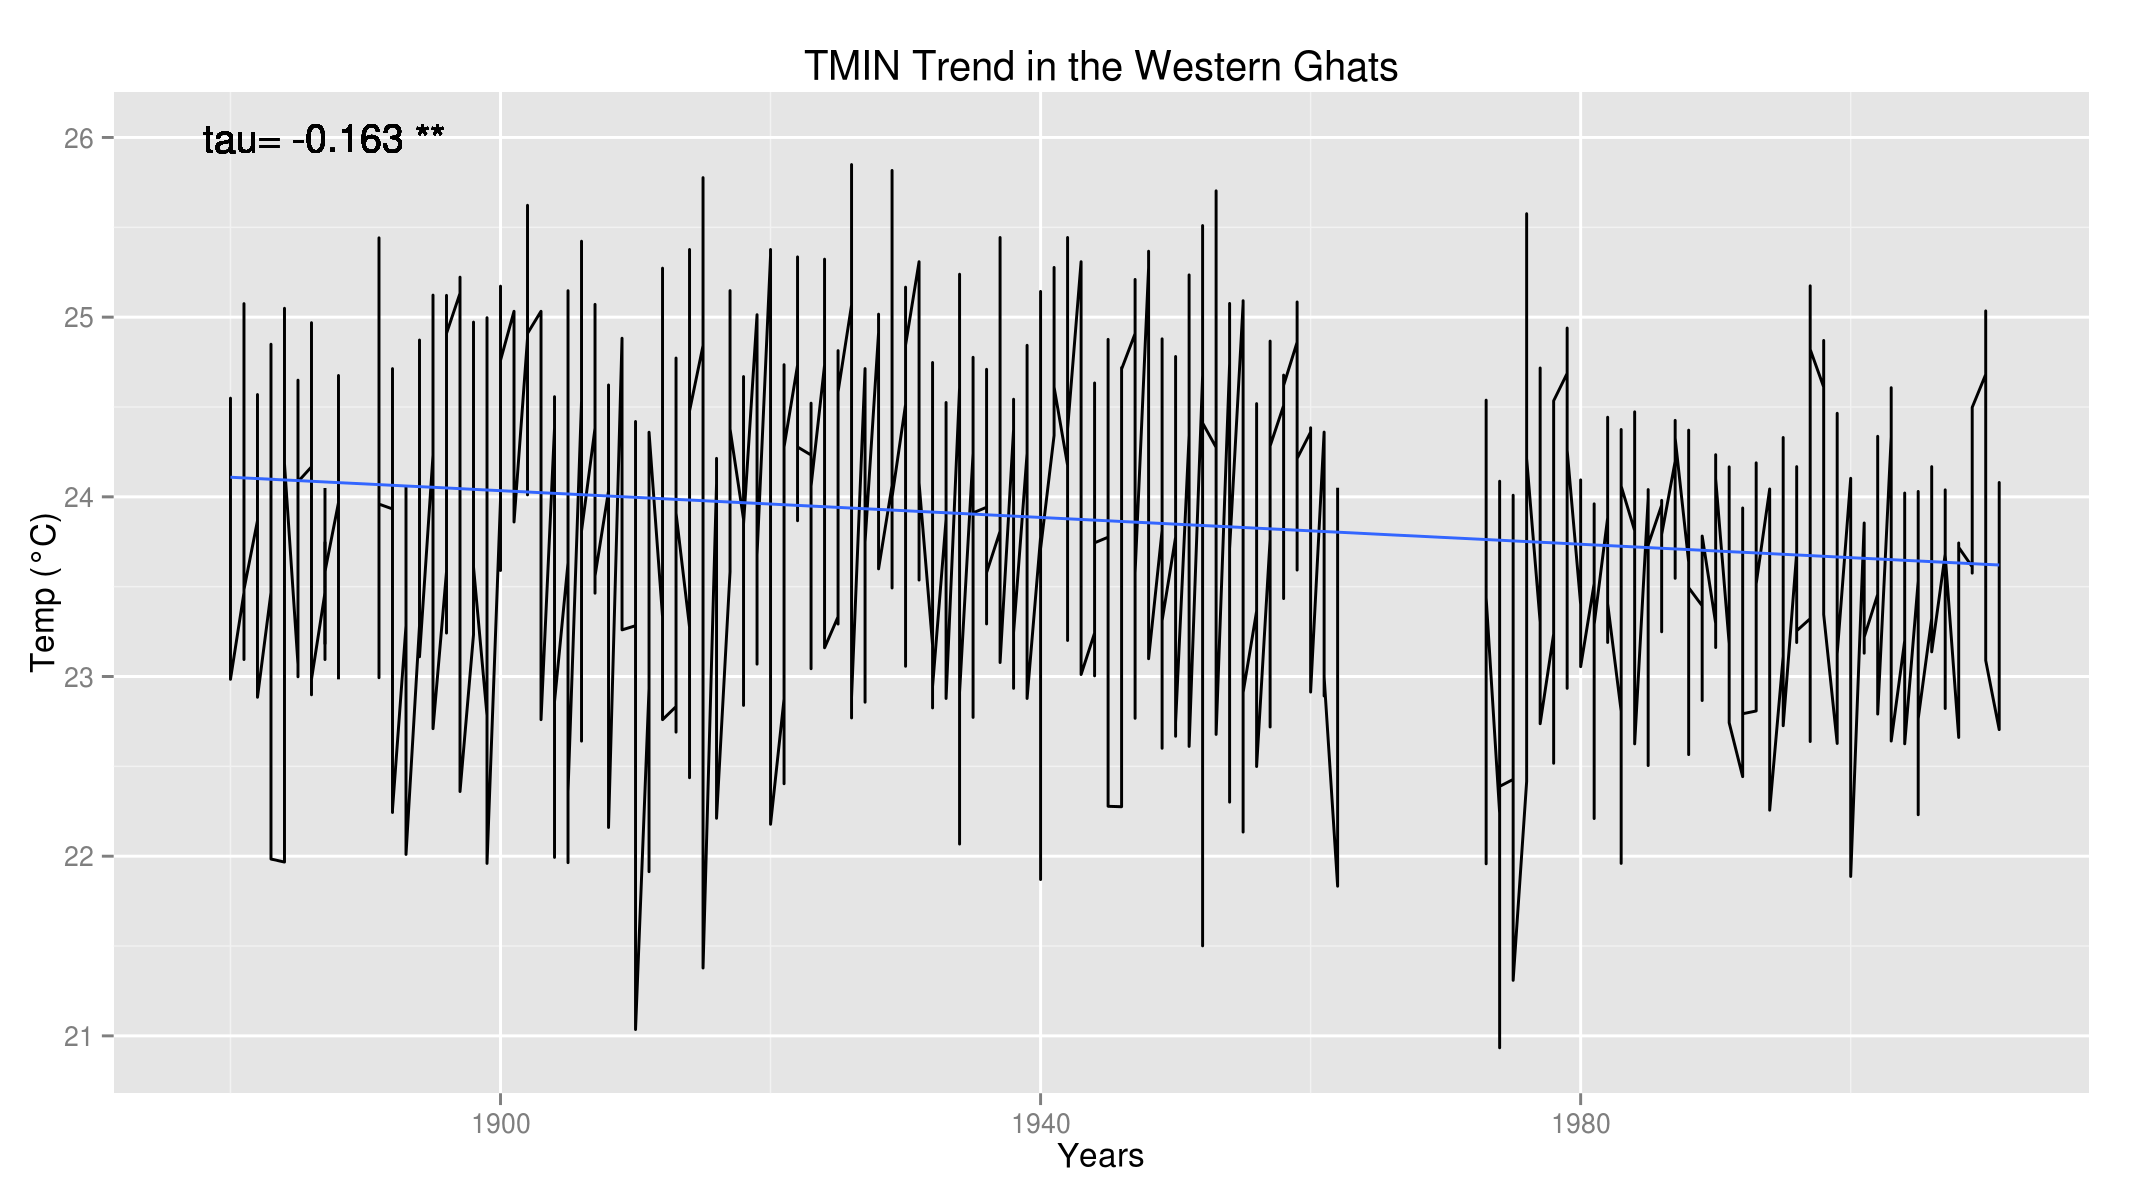
\includegraphics[width=5cm,height=2.7cm]{TMIN.png}\\
                    
  \end{tabular}
\captionof{figure}{\scriptsize Regional average temperature trend in the Western Ghats } 

  \end{minipage} 
 
 


%\multirow{4}{*}{BELGAUM}
% \hline
%\multirow{4}{*}{GOA/PANJIM} 
%\hline
%\multirow{4}{*}{NOVA GOA}
%\hline
%\multirow{4}{*}{MARMAGAO} 
% \hline
%\multirow{4}{*}{BANGALORE}&Average($^\circ$ C)&29.5$\pm$0.89&19.1$\pm$0.68&23.9$\pm$0.71\\ 
%&tau&0.196**& 0.22**&0.267**\\ \hline
%\multirow{4}{*}{MANGALORE/BAJPE}&Average($^\circ$ C)&31.7$\pm$0.73&23.0$\pm$0.6&27.0$\pm$0.58\\ 
%&tau&0.217**&-0.04&0.201**\\ \hline
%\multirow{4}{*}{MANGALORE}&Average($^\circ$ C)&30.5$\pm$0.68&23.5$\pm$0.67&27.0$\pm$0.61\\ 
%&tau& 0.057*&0.124**&0.118**\\ \hline
%\multirow{4}{*}{KOZHIKODE}&Average($^\circ$ C)&31.3$\pm$0.88&24.2$\pm$0.59&27.7$\pm$0.62\\ 
%&tau&0.499**&0.258**&0.396**\\ \hline
%\multirow{4}{*}{COIMBATORE/PEELAMED}&Average($^\circ$ C)&32.4$\pm$0.94&21.5$\pm$0.65&26.4$\pm$0.71\\ 
%&tau& 0.082*&0.199**&0.156**\\ \hline
%\multirow{4}{*}{FORT COCHIN}&Average($^\circ$ C)&31.1$\pm$0.69&24.2$\pm$0.59&27.3$\pm$0.54\\ 
%&tau& 0.084*& 0.087*&0.059**\\ \hline
%\multirow{4}{*}{THIRUVANANTHAPURAM}&Average($^\circ$ C)&31.4$\pm$0.89&23.6$\pm$0.47&27.0$\pm$0.68\\ 
%&tau&0.429**&0.059&0.476**\\ \hline
%\end{tabular}

\begin{tabular}{|c|c|c|c|c|}\hline 
\multicolumn{2}{|c|}{Stations} & TMAX & TMIN & TAVG \\ \hline 
\multirow{4}{*}{SURAT}&Average($^\circ$ C)&31.6$\pm$1.12&18.1$\pm$1.21&27.4$\pm$ 0.80\\
 &tau&0.013&0.032&0.028\\ \hline
\multirow{4}{*}{BOMBAY/SANTACRUZ}&Average($^\circ$ C)&31.9$\pm$ 1.03&22.6$\pm$ 0.85&27.1$\pm$0.85\\
 &tau&0.338**&0&0.288**\\ \hline
\multirow{4}{*}{BOMBAY / COLA}&Average($^\circ$ C)&31.7$\pm$0.82&23.9$\pm$0.73&27.3$\pm$0.75\\ 
&tau&0.062&0.217**&0.283**\\ \hline
\multirow{4}{*}{PUNE}&Average($^\circ$ C)&31.5$\pm$1.08&18.0$\pm$1.56&24.9$\pm$0.91\\ 
&tau&0.185**&0&-0.04**\\ \hline
\multirow{4}{*}{RATNAGIRI}&Average($^\circ$ C)&30.1$\pm$0.87&22.2$\pm$0.81&26.8$\pm$0.67\\ 
&tau&0.212**&-0.13**&0.03\\ \hline
\multirow{4}{*}{BELGAUM/SAMBRA}&Average($^\circ$ C)&30.2$\pm$0.96&18.4$\pm$1.04&24.3$\pm$0.67\\
 &tau&0.241**&-0.08**&0.058\\ \hline
\multirow{4}{*}{BELGAUM}&Average($^\circ$ C)&$\pm$&$\pm$&24.2$\pm$0.84\\ 
&tau&&&0.342**\\ \hline
\multirow{4}{*}{GOA/PANJIM}&Average($^\circ$ C)&31.6$\pm$0.79&23.4$\pm$0.75&27.4$\pm$0.66\\ 
&tau&0.241**&-0.01&0.222**\\ \hline
\multirow{4}{*}{NOVA GOA}&Average($^\circ$ C)&31.5$\pm$0.85&23.1$\pm$1.13&27.3$\pm$0.84\\ 
&tau&-0.30**&-0.09**&-0.23**\\ \hline
\multirow{4}{*}{MARMAGAO}&Average($^\circ$ C)&29.7$\pm$0.84&23.7$\pm$0.79&26.7$\pm$0.72\\ 
&tau&-0.14**&-0.07**&-0.11**\\ \hline
\multirow{4}{*}{BANGALORE}&Average($^\circ$ C)&29.5$\pm$0.89&19.1$\pm$0.68&23.9$\pm$0.71\\ 
&tau&0.196**& 0.22**&0.267**\\ \hline
\multirow{4}{*}{MANGALORE/BAJPE}&Average($^\circ$ C)&31.7$\pm$0.73&23.0$\pm$0.6&27.0$\pm$0.58\\ 
&tau&0.217**&-0.04&0.201**\\ \hline
\multirow{4}{*}{MANGALORE}&Average($^\circ$ C)&30.5$\pm$0.68&23.5$\pm$0.67&27.0$\pm$0.61\\ 
&tau& 0.057*&0.124**&0.118**\\ \hline
\multirow{4}{*}{KOZHIKODE}&Average($^\circ$ C)&31.3$\pm$0.88&24.2$\pm$0.59&27.7$\pm$0.62\\ 
&tau&0.499**&0.258**&0.396**\\ \hline
\multirow{4}{*}{COIMBATORE/PEELAMED}&Average($^\circ$ C)&32.4$\pm$0.94&21.5$\pm$0.65&26.4$\pm$0.71\\ 
&tau& 0.082*&0.199**&0.156**\\ \hline
\multirow{4}{*}{FORT COCHIN}&Average($^\circ$ C)&31.1$\pm$0.69&24.2$\pm$0.59&27.3$\pm$0.54\\ 
&tau& 0.084*& 0.087*&0.059**\\ \hline
\multirow{4}{*}{THIRUVANANTHAPURAM}&Average($^\circ$ C)&31.4$\pm$0.89&23.6$\pm$0.47&27.0$\pm$0.68\\ 
&tau&0.429**&0.059&0.476**\\ \hline
\end{tabular}








\begin{table}[htbp]
    \caption{Table with gray and white.}
    \begin{center}
    \begin{tabular}{lcccl}
                                                                                    & Column 1      & Column 2      & Column 3                      & Column 4                      \\ \rowcolor{lightgray}
                                                                                    & PM            & 1             & 2                             & 28                            \\
    \multicolumn{1}{>{\columncolor{lightgray}}l}{}                                  & PD            & 3             & 4                             & 29                            \\ \rowcolor{lightgray}
                                                                                    & PM            & 5             & 6                             & 30                            \\
    \multicolumn{1}{>{\columncolor{lightgray}}l}{\multirow{-4}{*}{Gray}}            & PD            & 7             & 8                             & 31                            \\ \rowcolor{lightgray}


    \multicolumn{1}{>{\columncolor{white}}l}{}                                      & PM            & 9             & 10                            & 32                            \\
                                                                                    & PM            & 11            & 12                            & 33                            \\ \rowcolor{lightgray}
    \multicolumn{1}{>{\columncolor{white}}l}{}                                      & PD            & 13            & 14                            & 34                            \\
                                                                                    & PM            & 15            & 16                            & 35                            \\ \rowcolor{lightgray}
    \multicolumn{1}{>{\columncolor{white}}l}{\multirow{-5}{*}{White}}               & PD            & 17            & 18                            & 36                            \\


    \multicolumn{1}{>{\columncolor{lightgray}}l}{}                                  & P1            & 20            & 21                            & 37                            \\ \rowcolor{lightgray}
                                                                                    & P2            & 22            & 23                            & 38                            \\
    \multicolumn{1}{>{\columncolor{lightgray}}l}{}                                  & P3            & 24            & 25                            & 39                            \\ \rowcolor{lightgray}
    \multicolumn{1}{>{\columncolor{lightgray}}l}{\multirow{-4}{*}{Gray}}            & P4            & 26            & 27                            & 40                            \\

    \end{tabular}
    \end{center}
    \end{table}






\end{document}